\pagenumbering{arabic}
\section{Introduction}
\subsection{Overview}
Natural selection has different forms, distinguishing by the various effects on allele frequencies and the linkage between single nucleotide polymorphisms (SNPs). At a biallelic locus undergoing directional selection, the favorable allele will quickly become fixed in the gene pool of the population while the less favorable allele will be rapidly removed. On the other hand, selection in which multiple alleles at a locus are actively maintained in the gene pool of a population is termed balancing selection \citep{RN1}. Until now, relatively little attention has been devoted into this type of selection, especially in studies looking for signatures of evolution at a genome-wide scale \citep{RN2}. One of the reasons is that balancing selection partially contradicts with the classical view of evolution \citep{RN3}. Take the famous sickle-cell allele as an example, the balancing view states that the heterozygosity persists in populations through heterozygote advantage \citep{RN1}. In contrast, the classical view doesn’t attribute a major role to heterozygote advantage; proponents of the classic view believe that the heterozygosity of sickle-cell allele is a result of incomplete purifying selections \citep{RN1}. This controversy was not resolved until the middle of the twentieth century when the classical view was challenged by the detection of ample variation through allozyme electrophoresis \citep{RN3}. The classic view cannot explain the maintenance of such large amounts of genic heterozygosity, though the idea of pervasive balancing selection is also hard to defend.

Today, even though most people agree with the existence of balancing selection, the community is still contentious about its prevalence \citep{RN2}. Researchers are equivocal about whether balancing selection is rare, or there is simply no efficient technique to detect it. One of the main reasons is that not every allele polymorphism is considered the result of balancing selection. In order to constitute balancing selection, each allele involved in the allele polymorphism should have a statistically higher allele frequency than expected from random processes, including mutation, recombination, and genetic drift. Because population statistics are necessary for removing minor allele polymorphisms, detection of balancing selection requires analysis of population-level genome data, which has been difficult to obtain until recently.

Apart from the uncertainty in prevalence, balancing selection also has intrinsic reasons to be studied. After all, many evolutionary processes are based on genetic variations. While mutation is the ultimate source of genetic diversity, balancing selection may be an important mechanism to maintain this diversity. The change of vesicular monoamine transporter I during human evolution is an example of how balancing selection maintains the diversity of some human genes \citep{RN4}. Originally, this protein underwent directional selection in which a threonine replaced the asparagine at position 136. However, after ancient humans went out of Africa, another point substitution occurred, and balancing selection maintained both the threonine and a new isoleucine allele of this protein in modern human populations \citep{RN4}. Clearly, studying balancing selection will help people better recreate evolutionary paths of human and other organisms, which has significant meanings in understanding current as well as predicting future evolutionary trends.

\subsection{Study system}
\emph{Capsella grandiflora} is a species of flowering plant in the Brassicaceae family. It is referred to by the common name grand shepherd's-purse. The main signature of this plant compared to other \emph{Capsella} species is its wide flower petals. \emph{C. grandiflora} is mainly distributed in south European countries such as Greece and Italy. However, its close relative, \emph{Capsella rubella}, is found in many other places including the North America, and it is also closely related to \emph{Arabidopsis thaliana}. The close evolutionary relationships between these other species and \emph{C. grandiflora} allow the use of genetic tools and resources developed for these species when studying \emph{C. grandiflora}. \emph{C. grandiflora} is not the most common plant model used in genomic studies, but it has a large and stable effective population size, which means selection signatures will be strong and not be overly distorted by demographic factors \citep{RN6}. A previous study done by \citet{RN7} confirmed the existence of balancing selection in the genus of \emph{Capsella}. This work found that signatures of balancing selection were maintained at disease resistance loci following mating system shifts in \emph{C. rubella}. Besides, \citet{RN8} showed that long-term balancing selection has driven the evolution of immunity in \emph{Capsella orientalis}. Therefore, if balancing selection is common, \emph{C. grandiflora} will be a promising species where the signals will be strong, which may mitigate the difficulty of distinguishing balancing selection signals from other selection signatures.

\subsection{Short-term balancing selection}
The specific type of balancing selection investigated in this study is short-term balancing selection, which is ongoing selection or selection occurred relatively recently with respect to evolutionary timescale \citep{RN2}. The main reason to choose to study short-term balancing selection is because it is most relevant to humans. Investigating atmospheric changes that occurred millions years ago may not have significant meanings to people today, but studying the spread of an agricultural disease that occurred hundreds years ago, for example, may help researchers prevent future outbreaks with similar pathogens. Besides, the detection of short-term balancing selection requires minimum data input. For long-term balancing selection, one of the signatures, for instance, is trans-species polymorphism \citep{RN2}. Detection of this kind of polymorphism requires genomic data of multiple closely related species. On the other hand, short-term balancing selection is featured by high genetic variations and extended linkage disequilibrium (LD) \citep{RN2}. Investigating the genomic data of many individuals from a single population will be sufficient to reach a conclusion regarding to signals of this type of selection. Consequently, this study focused on detecting evidence of short-term balancing selection in \emph{C. grandiflora}.

\section{Materials and Methods}
\subsection{Genome data}
The eight chromosome VCFs were provided by Dr. Josephs at the Department of Plant Biology, Michigan State University. The data contained the genetic information of 177 \emph{C. grandiflora} individuals sampled from Greece and grown in the greenhouse at the University of Toronto. The sample preparation, extraction, and genotyping details can be found in \citet{RN11}. For this research, \emph{C. grandiflora} SNP sites were selected from the genome data, while invariant and variant sites were filtered based on genotyping quality to ensure the data was available for all samples. Reads were aligned to the \emph{C. rubella} reference genome, and multiallelic sites as well as indels were removed from the resulting variant sites. Those VCFs were then phased separately using a combination of read-backed and population level phasing, including IBD2 blacklisting with default parameters and a phase error rate of 0.0001 (Kent, 2022). The \emph{C. rubella} reference genome version 1.1 from Phytozome (https://phytozome-next.jgi.doe.gov/)  was used to identify genes and the corresponding \emph{A. thaliana} gene orthologues.

\subsection{The Tajima’s test}
The Tajima’s test is a population statistic test created by and named after Japanese researcher Fumio Tajima. The score of this test, Tajima's D (\emph{D}), is computed as the difference between the mean number of pairwise differences and the number of segregating sites, each scaled so that they are expected to be the same in a selection-free population of constant size \citep{RN12}. Tajima’s D distinguishes between an allele evolving randomly and one evolving under a non-random process. One common way of interpreting the score is to see positive score as the sign for balancing selection and negative score as the sign for directional selection \citep{RN12}. Though, other demographic factors can also explain variations in \emph{D} (e.g. population size changes). The first step of the Tajima’s test is to calculate the pairwise differences (\emph{k}), also known as the nucleotide diversity. The pairwise differences measures the genetic variation within a population. It is defined as the average number of nucleotide differences per site between two DNA sequences in all possible pairs in the sample population \citep{RN13}. However, as mentioned previously, polymorphisms maintained by balancing selection should have a statistically higher frequency than expected from mutation, recombination, or genetic drift. Pairwise differences itself is not sufficient to eliminate allele polymorphisms resulted from non-selection processes. In full, Tajima’s D is shown below:

\begin{equation}
D=\frac{k-\frac{s}{6.4452}}{\sqrt{0.0279\times S+0.0025\times S(S-1)}}
\end{equation}

\noindent where the constants are determined based on the sample size (354) following the descriptions in the Tajima’s paper (1989) and S is the number of segregating sites. In conclusion, Tajima’s D is a balancing selection indicator because it eliminates insignificant allele polymorphisms using the population statistics.

In this study, the pairwise differences of each SNP site was directly read from the chromosome VCFs. In total, there were 177 diploid individuals, so the sample size was 354 assuming each individual provided two independent samples. To better avoid signals resulted from recombination, each chromosome was parsed into windows with a constant window size of 100 SNP sites based on the linkage disequilibrium in \emph{C. grandiflora} \citep{RN11}. By doing so, the pairwise differences of each widow was the sum of pairwise differences of the included SNP sites, and the number of segregating site was always 100 except the last window at the end of each chromosome. The Tajima’s Ds of these windows were plotted against their base pair positions. The top 50 windows with highest \emph{D} values were selected and converted to gene candidates using the \emph{C. rubella} reference genome, and their associated biological functions were investigated using \emph{A. thaliana} gene orthologues.

\subsection{The extended haplotype homozygosity (EHH) test}
The EHH test is a population statistic test designed to detect directional selection in a population \citep{RN14}. It relies on the relationship between an allele's frequency and the linkage disequilibrium between that allele and the loci that surround it. If there is no selection, new alleles take a long time to increase in frequency, and recombination around them will ensure that blocks of LD decay over time. By contrast, in the presence of selection, especially directional selection, young alleles will spread rapidly through the population and will be surrounded by long blocks of LD, as there would not have been enough time for recombination to erode them. Specifically, in the EHH test, the decay of LD around each core haplotype is assessed by adding more and more distant SNP sites. This allows the calculation of the probability that any two chromosome segments that carry a given core haplotype are identical by descent \citep{RN14}.

In this study, the EHH test was used to detect evidence of balancing selection on 28 of the 50 windows from the Tajima’s test. The rest 22 windows were not testable due the limit of the Selscan program \citep{RN15}. Apart from the LD decay curves, the results of the EHH test were plotted as colormaps in which haplotypes that are identical by descent were drew with the same color. Instead of a dominant color (directional selection), if there are multiple color clusters shown on the colormap, the window is believed to undergo balancing selection since color clusters indicate allele polymorphisms consistent with balancing selection.

\subsection{The integrated haplotype homozygosity pooled (iHH12) test}
Based on idea of LD decay, \citet{RN16} designed the iHH12 test, which can be considered an integrated version of the EHH test. The iHH12 test has two scores depending on whether it is computed with respect to the ancestral or derived core allele. When the rate of EHH decay is similar on the ancestral and derived alleles, it indicates no selection and therefore the iHH12 score will be close to 0. Large negative values indicate unusually long haplotypes carrying more on the derived allele, which are indicators of directional selection, and large positive values indicate long haplotypes carrying more on the ancestral allele, which are signs for balancing selection \citep{RN16}. The iHH12 score is also constructed to have an approximately standard normal distribution, hence the sizes of iHH12 signals from different SNP sites are directly comparable regardless of the allele frequencies at those sites \citep{RN16}. In conclusion, the iHH12 test provides a measure of how unusual the haplotypes around a given SNP site are relative to the genome as a whole, without a formal significance test.

In this study, the whole genome data was run through the iHH12 test, with an assumption of uniform recombination possibility across each chromosome. Similar to the Tajima’s test, the iHH12 scores were plotted against their base pair positions.

\subsection{The gene ontology (GO) enrichment analysis}
The GO enrichment analysis (\url{http://geneontology.org/}) is based on the PANTHER (protein annotation through evolutionary relationship) classification system designed by \citet{RN17}, which combines gene function, ontology, pathways, and statistical analysis tools to analyze genome-wide data. The p-value of this analysis is the probability of seeing significant number of genes out of the total gene inputs to a particular GO term, given the proportion of genes in the whole genome that are annotated to that GO term \citep{RN17}. The closer the p-value is to zero, the more significant the particular GO term associated with the group of genes is. For instance, if all of the genes in a group are associated with “disease resistance”, this term will be significant. However, since all genes in the genome are indirectly associated with the top level term “homeostasis”, this will not be significant if all the genes in a group are associated with this very high level term.

In this study, the top 50 windows from the Tajima’s test were found to associate with 46 different genes using \emph{A. thaliana} gene orthologues, which are included in the \emph{C. rubella} reference genome mentioned previously. The list of these 46 gene orthologues was used as the input of the GO enrichment analysis. Biological functions and corresponded p-values were automatically generated by the PANTHER system.

\subsection{Custom Code}
All the python and bash codes, as well as analysis details, can be found on \url{https://github.com/FergusonZhang/Thesis}. The Selscan package (\url{https://github.com/szpiech/selscan}), include the EHH and the iHH12 algorithms, is explained in \citet{RN15}.

\section{Results}
\subsection{The Tajima maps}
Tajima’s D with a window size of 100 SNP sites were calculated and plotted against their base pair positions on the corresponded chromosome. Since the Tajima’s test was a scaled test, the scores of the whole genome (all eight chromosomes) were put together for comparison, and the top 50 windows with highest \emph{D} values were selected. \cref{fig:1} on the next page shows the results of the Tajima’s test. The purpose of performing the Tajima’s test was to identify balancing selection candidate regions that generated the strongest signals. These 50 windows were later compared with the results of other tests to eliminate potential “false positives” since balancing selection is not the only force that can produce a high Tajima’s D \citep{RN12}. According to the maps, there were more than 50 windows that had positive \emph{D} values, which suggested a large proportion of the \emph{C. grandiflora} genome contains SNPs with higher frequency than expected from chance. Traditionally, a significance test would be performed, and a confidence interval (CI) would be created to winnow positive outliers. However, in this case, there were millions of windows in total, so a CI would still generate thousands of outliers, which were too many to be studied. Since the large proportion of the genome with positive \emph{D} values already agreed with the existence of balancing selection in \emph{C. grandiflora}, only the windows that could generate strong selection signatures were worthy to be further analyzed. Consequently, only the top 50 windows were selected, and these 50 windows were found to be not uniformly distributed in the \emph{C. grandiflora} genome.

\begin{figure}[h!]
    \centering
    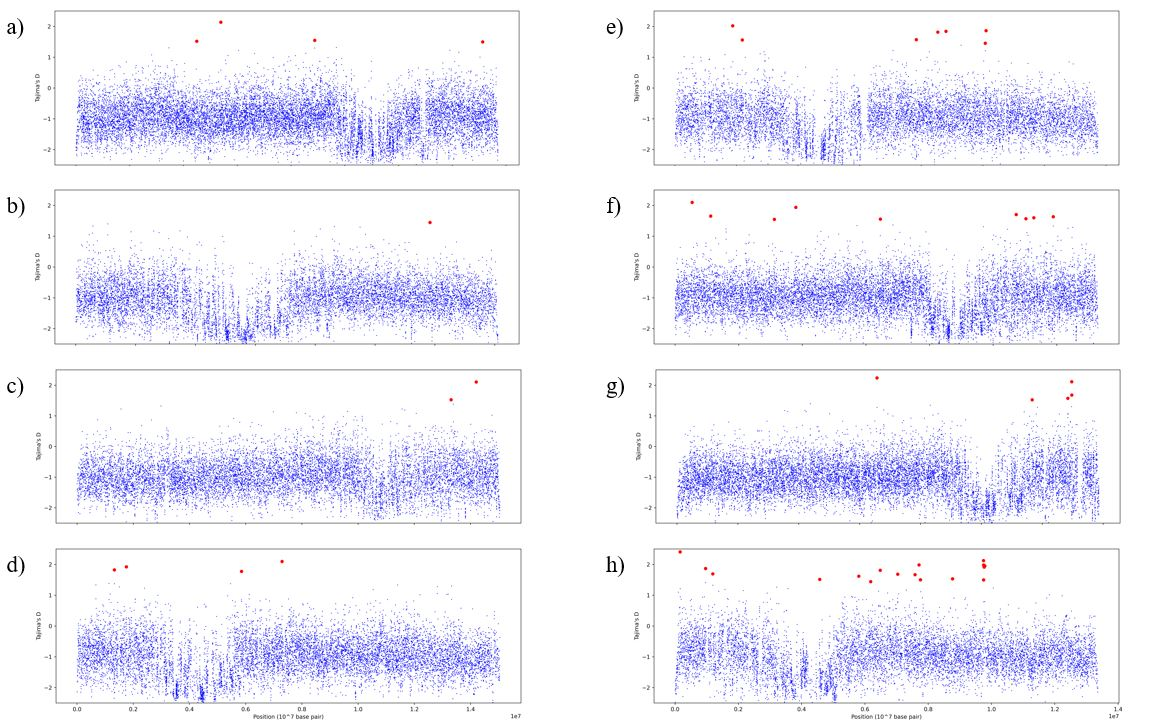
\includegraphics[scale=0.7]{figs/1.JPG}
    \caption{The Tajima maps of chromosome 1-8 (a-h). The x-axis is the base pair position with a unit of 10 million nucleotides, and the y-axis is the Tajima’s D. The top 50 windows are marked with red dots. The top 50 windows all have \emph{D} values $\geq$ 1.3714. Detailed maps are included in the supplementary materials.}
    \label{fig:1}
\end{figure}

\subsection{Gene candidates}
To investigate the kinds of genes in \emph{C. grandiflora} which identified as candidates for balancing selection, the top 50 windows were converted to genes based on their proximity to genes in the \emph{C. rubella} reference genome. Specifically, each window was aligned to the gene(s) that located entirely or partially in the 100 SNP window. These 50 windows were found to be associated with 46 different genes. The 46 gene candidates were then converted to their \emph{A. thaliana} gene orthologues for function analysis since \emph{A. thaliana} was a well-studied plant species close to the \emph{Capsella} genus, and its genes were recorded in the PANTHER system for the GO enrichment analysis \citep{RN17}. These 46 gene candidates were found to cover a variety of biological functions, mainly including metabolism, disease resistance, immune response, and membrane transportation. The table of position, gene, and biological function can be found in the online supplementary information on github (\url{https://github.com/FergusonZhang/Thesis/blob/main/Results/Gene\%20candidates\%20and\%20functions.xlsx}). \cref{fig:2} on the next page shows the corresponded gene to the window with the largest Tajima’s D on chromosome 7, Scaffold7:8200257.

\begin{figure}[h!]
    \centering
    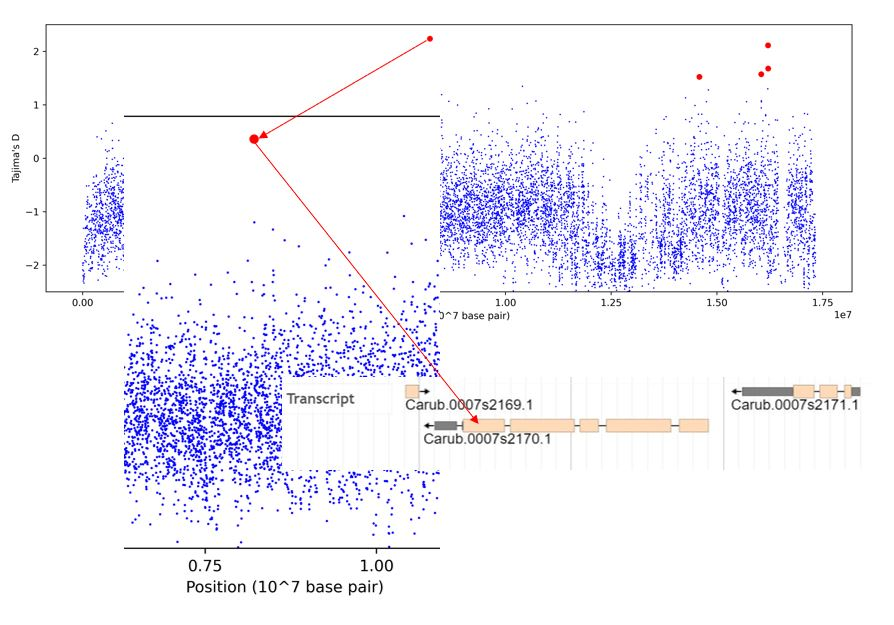
\includegraphics[scale=0.7]{figs/3.JPG}
    \caption{The window Scaffold7:8200257 on chromosome 7. Its corresponded \emph{C. rubella} gene is Carub.0007s2170. The transcript screenshot is from the \emph{C. rubella} genome JBrowse (\url{https://phytozome-next.jgi.doe.gov/info/Crubellav11}).}
    \label{fig:2}
\end{figure}

The corresponded \emph{C. rubella} gene of Scaffold7:8200257, Carub.0007s2170, encodes disease resistance protein RPP2B, which cooperates with RPP2A to confer resistance to \emph{Hyaloperonospora parasitica} \citep{RN18}. \emph{H. parasitica} is an oomycete from the family Peronosporaceae. It has been considered for a long time to cause downy mildew of a variety of species within the Brassicaceae family, on which the disease could cause serious damage by killing seedlings or affecting the quality of produce intended for freezing \citep{RN18}. The high Tajima’s D on this gene was consistent with the previous finding that disease resistance was one of the major selective forces of balancing selection.

\subsection{The iHH12 maps}
Similar to the Tajima’s test, the scores of the iHH12 test \citep{RN16} were plotted against their base pair positions on the corresponded chromosome. However, the background noise was much greater using this analysis relative to the Tajima’s test. As a result, the top 50 windows from the Tajima’s test were hardly outliers on the iHH12 maps (none of the top 50 windows was among the top 500 peaks of the iHH12 test). One contributing reason for this difference was the assumption that recombination was uniform across each chromosome. This assumption was not always true. For instance, at the centromere, recombination possibility should be very close to zero due to its physical conformation during meiosis. Unfortunately, the recombination possibility map of \emph{C. grandiflora} was not available for this study, so the uniform recombination possibility was assumed.

\begin{figure}[h!]
    \centering
    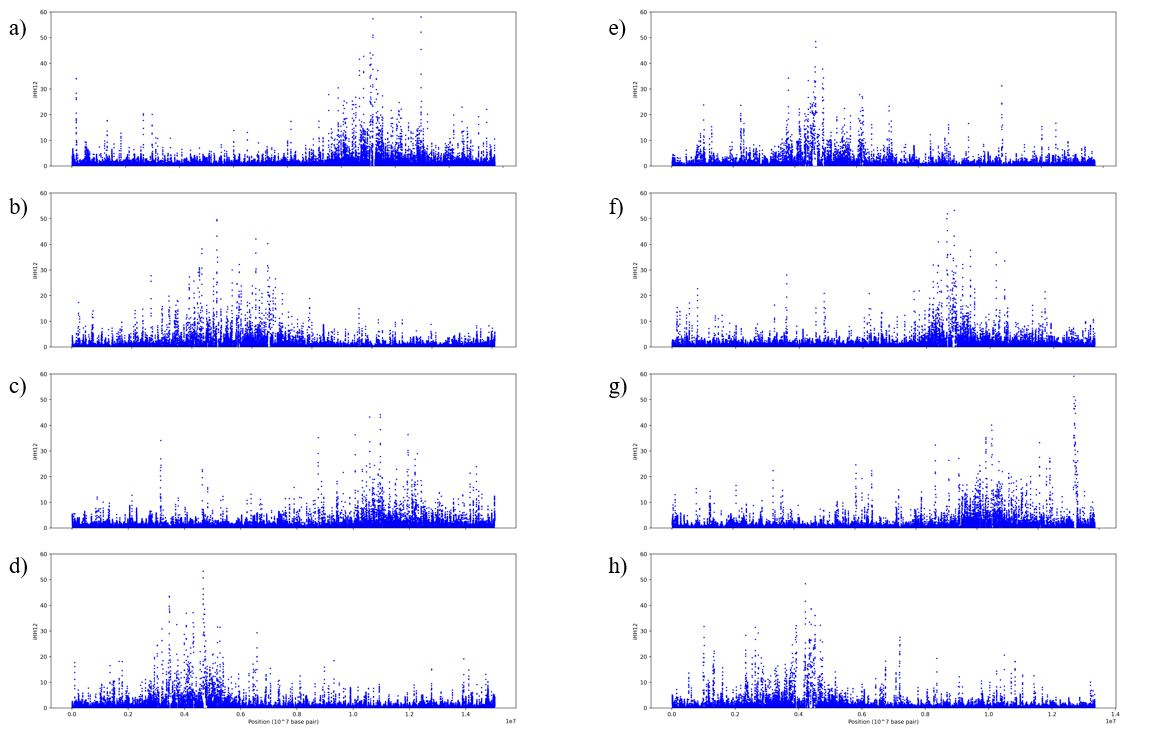
\includegraphics[scale=0.7]{figs/2.JPG}
    \caption{The iHH12 maps of \emph{C. grandiflora} chromosome 1-8 (a-h). The x-axis is the base pair position with a unit of 10 million nucleotides, and the y-axis is the iHH12 score. Detailed maps are included in the supplementary materials.}
    \label{fig:3}
\end{figure}

Even though the top 50 windows form the Tajima’s test were no longer outliers on the iHH12 maps, corresponded local peaks were still observed for all the 50 windows as conformations of the evidence of balancing selection in \emph{C. grandiflora}. The iHH12 test is a test designed for positive sweeps, so the a high iHH12 score doesn’t necessarily refer to balancing selection. For instance, an incomplete or ongoing directional selection could also yield a high iHH12 score \citep{RN16}. As a result, using the iHH12 score as a double check for the Tajima’s D is safer than using it as an independent balancing selection indicator. On page 9, there are the Tajima and iHH12 maps of Scaffold7:8200257, the example window mentioned in the gene candidate section. Despite the noise around the centromere, a local peak was still observed on the iHH12 map as the evidence of balancing selection.

\begin{figure}[h!]
    \centering
    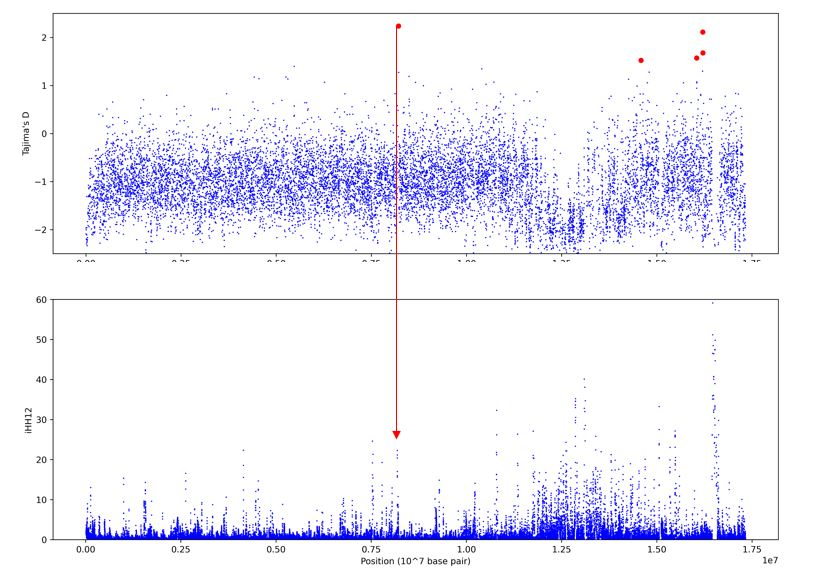
\includegraphics[scale=0.8]{figs/4.JPG}
    \caption{The Tajima and iHH12 maps of \emph{C. grandiflora} chromosome 7. The window Scaffold7:8200257 is identified on both maps as a potential region for balancing selection.}
    \label{fig:4}
\end{figure}

\subsection{The EHH decay curves and haplotype colormaps}
As discussed in the introduction, the two features of short-term balancing selection are high genetic variations and extended haplotypes \citep{RN2}. The EHH test could visually reflect the idea of extended haplotypes by plotting the EHH decay curves as well as haplotype colormaps centered at a specific locus \citep{RN14}. Therefore, in order to further validate the results of the Tajima’s test, the top 50 windows were run through the EHH test. However, since the VCFs only contained SNP sites, not all the 50 windows had successfully generated interpretable results due to the limit of the Selscan program \citep{RN15}. Specifically, only 28 of the 50 windows were testable. All the 28 EHH decay curves as well as the 28 haplotype colormaps can be found in the online supplementary information on github (\url{https://github.com/FergusonZhang/Thesis/tree/main/Results/The\%20EHH\%20test}).

\begin{figure}[h!]
    \centering
    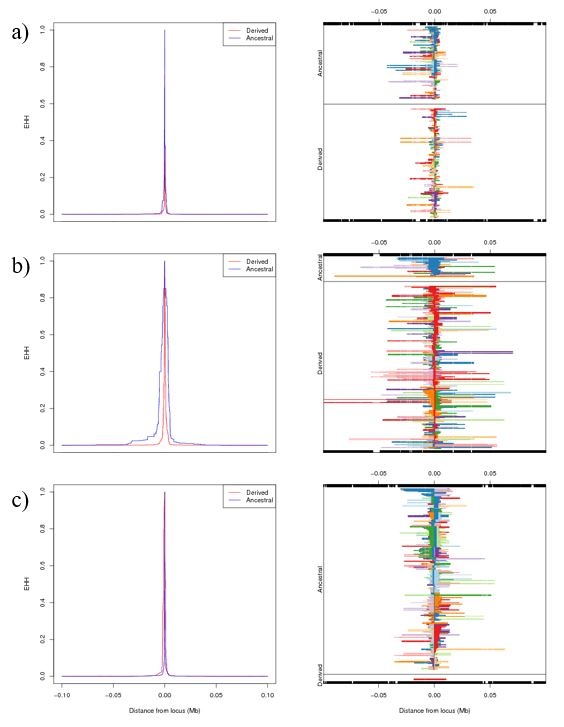
\includegraphics[scale=1]{figs/5.JPG}
    \caption{Representative EHH decay curves and haplotype colormaps from three Tajima’s D windows identified earlier. a) Scaffold6:13784825 on chromosome 6, an example of neutral evolution, b) Scaffold8:9789743 on chromosome 8, an example of possible directional selection, and c) Scaffold4:1753945 on chromosome 4, an example of possible balancing selection. The zero of the x-axis is centered at the window with a unit of 1 million nucleotides. The y-axis of the EHH decay curve is the possibility of observing the haplotype.}
    \label{fig:5}
\end{figure}

When the rate of EHH decay is similar on the ancestral and derived alleles, it indicates no selection. Slower decay of the ancestral allele is a sign for directional selection, and slower decay of the derived allele is a sign for balancing selection \citep{RN14}. In the colormaps, haplotypes that are identical by descent were marked with the same color. If there is no dominant color, it indicates no selection at this window. If there is a dominant color, then directional selection is believed to occur. If there are multiple color clusters, it is a sign for balancing selection. Among the 28 testable windows, all the three potential outcomes of the EHH test were observed. For example, as shown in part a) of \cref{fig:5}, for the window Scaffold6:13784825 on chromosome 6, the ancestral and derived decay rate were about the same, and no dominant color was observed in either of the alleles. All these characteristics indicated no selection occurred on this window. On the other hand, as shown in part b) of \cref{fig:5}, the window Scaffold8:9789743 on chromosome 8 had features for directional section. The ancestral decay rate was smaller than the derived decay rate, and both alleles had a dominate haplotype (blue for ancestral, red for derived). Finally, as shown in part c) of \cref{fig:5}, the window Scaffold4:1753945 on chromosome 4 supported the existence of balancing selection. The rate of EHH decay was smaller on the derived allele, and at least five common haplotypes were observed (blue, green, light blue, orange, and red). Even though not all the 28 testable windows generated balancing selection-like results, the existence of windows like Scaffold4:1753945 was consistent with the existence of balancing selection in \emph{C. grandiflora}.

\subsection{The GO enrichment analysis}
Using \emph{A. thaliana} as the organism template, the GO enrichment analysis didn’t find any specific biological function that the 46 gene candidates were associated with (all p-values were much smaller than 0.05, the derailed table can be found in the online supplementary information on github (\url{https://github.com/FergusonZhang/Thesis/blob/main/Results/GO\%20enrichment\%20analysis\%20results.xlsx}).). In other words, the short-term balancing selection in \emph{C. grandiflora} was very likely resulted from a variety of reasons.

\section{Discussion}
In this study, the genome data of 177 individuals from a single \emph{C. grandiflora} population was used to detect evidence of short-term balancing selection in this plant species. The data was filtered and phased, containing only biallelic SNP sites that shared by all of the 177 individuals. This simplification provides convenience for coding and computational analysis; however, it also increases the chance of missing important balancing selection signals because multiallelic SNP sites may be as important as biallelic SNP sites in signal detection. For instance, multiallelic SNP sites can produce high genetic variation signals that recognized by the Tajima’s test \citep{RN12}. They could also be important components of core haplotypes on the ancestral or derived allele, which can directly affect the EHH decay rate, haplotype colormaps, as well as the iHH12 test score \citep{RN15}. Since balancing selection is likely to maintain several alleles at a locus, we might expect loci experiencing balancing selection to be enriched for multiallelic SNP sites. By excluding these sites, we likely reduce the signals of balancing selection in our data, making our tests using only biallelic sites conservative. This contrast also helps justify only investigating the top 50 windows from our analyses: since these are the strongest signals of possible balancing selection, they are more likely to be true signals. Additionally, since biallelic SNP sites covered almost the entire genome of \emph{C. grandiflora}, our analyses also have high coverage across the entire genome, and the purpose of detecting evidence of short-term balancing selection in \emph{C. grandiflora} was still fulfilled.

The Tajima’s test can not only reflect genetic variations within a population, but also reduce the effects of minor allele polymorphisms resulted from neutral processes. Therefore, it was chosen as the primary indicator of balancing selection in this study, despite the fact that directional selections may also yield high Tajima’s Ds \citep{RN12}. Fortunately, we have the EHH and the iHH12 tests that can function as double checks of balancing selection, and we will discuss them later. To further avoid high \emph{D} values resulting from recombination, the genome was parsed into windows of 100 SNP sites, and this parsing is reasonable because the expected linkage disequilibrium in \emph{C. grandiflora} is about the same size \citep{RN11}. As explained in the section of the Tajima maps, we didn’t apply any statistical test to the Tajima’s Ds because of the gigantic data size. The top 50 windows with highest \emph{D} values were selected since they were believed to contain strongest selection signatures. Thanks to the evolutionary similarities, the conversion of windows to gene candidates using the \emph{C. rubella} reference genome can be well-explained, and the GO enrichment analysis using \emph{A. thaliana} gene orthologues are also justifiable. The only concern regarding to this series of conversion is that \emph{A. thaliana} is a selfer while \emph{C. grandiflora} and \emph{C. rubella} are crossers. According to \citet{RN1}, the self-incompatibility (SI) locus is more likely to undergo balancing selection in a crosser than in a selfer. This is because under animal or wind pollination, rare pollen and pistil types could produce better genetic outputs in crossers \citep{RN1}. However, since the SI locus is still present in \emph{A. thaliana}, the \emph{C. grandiflora} data was aligned successfully, and positive Tajima’s Ds were observed around the SI locus (base pair 9989743-10174325, chromosome 8). In conclusion, this series of conversion is justifiable and necessary since neither \emph{C. grandiflora} nor \emph{C. rubella} is registered for the PANTHER system of the GO enrichment analysis \citep{RN17}.

The iHH12 test takes a recombination possibility map as one of its inputs \citep{RN16}. Unfortunately, the recombination possibility map of \emph{C. grandiflora} was not available for this study, so we assumed the recombination possibility was uniform across each chromosome. The result was a strong background noise of the iHH12 score. Fortunately, we still observed local peaks on the iHH12 maps that corresponded to all the top 50 windows from the Tajima’s test, suggesting balancing selection occurred on the \emph{C. grandiflora} genome. Similarly, the EHH test \citep{RN14}, even though could only run on 28 of the 50 windows, had successfully generated evidence supporting the existence of balancing selection. Both the EHH test and the iHH12 test are designed for directional selections, so using them as peripherals of the Tajima’s test is an acceptable solution.

All the p-values generated by the GO enrichment analysis were found to be much smaller than 0.05, indicating that the gene candidates under balancing selection were not resulted from a single selective force. This wide coverage of selective forces was expected for balancing selection \citep{RN1}. Any dynamic or oscillating environmental factor (e.g. disease, temperature fluctuations, available nutrition) could be the source of balancing selection since it provides a chance for different phenotypes to compete with each other with varying fitness, maintaining the allele polymorphisms inside the population. Observing this wide coverage further confirmed the existence of balancing selection in \emph{C. grandiflora}.

\section{Conclusion}
The results of the Tajima’s test, the iHH12 test, and the EHH test were consistent with the existence of short-term balancing selection in \emph{C. grandiflora}, and those gene candidates under balancing selection were found to involve in a variety of biological functions, including membrane transportation, disease resistance, immune response, and metabolism. In the future, the genome data of \emph{C. grandiflora} containing both biallelic and multiallelic SNP sites should be used for the detection of balancing selection signals, and the recombination possibility map of \emph{C. grandiflora} should be incorporated in the iHH12 test for noise reduction. When the annotated \emph{C. grandiflora} genome is available, potential genes under balancing selection should be directly analyzed using the PANTHER system to better investigate potential selective forces of balancing selection in \emph{C. grandiflora}.